%
% Prusa.tex
%
% History of LulzBot Printers
%
% Copyright (C) 2014, 2015 Aleph Objects, Inc.
%
% This document is licensed under the Creative Commons Attribution 4.0
% International Public License (CC BY-SA 4.0) by Aleph Objects, Inc.
%

\begin{figure}[h!]
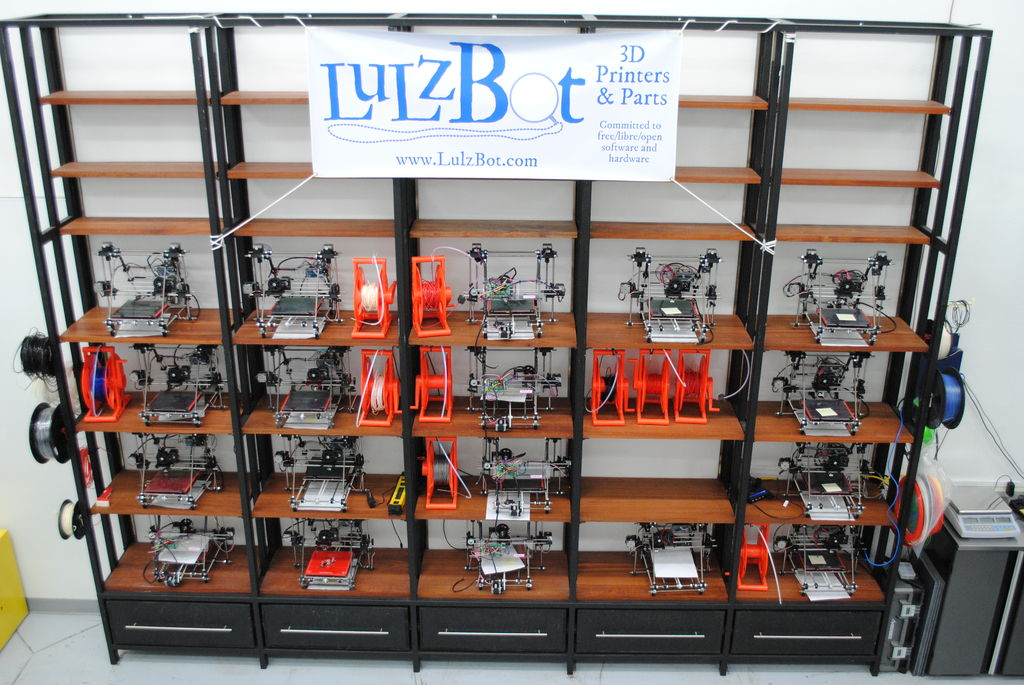
\includegraphics[keepaspectratio=true,height=0.40\textheight,width=1.00\textwidth,angle=0]{prusa/prusa-display.jpg}
 \caption{LulzBot Prusas.}
 \label{fig:prusa-display}
\end{figure}

The LulzBot Prusas were based on the Prusa Mendel design. The Prusas
printed more Prusas and they printed the LulzBot AO-100s. Approximately
128 Prusas were built. Prusa Version 1.0 production started in the first
quarter of 2011. Version 2.0 production started in the second quarter of 2011.

%
% Prusa.tex
%
% History of LulzBot Printers
%
% Copyright (C) 2014, 2015 Aleph Objects, Inc.
%
% This document is licensed under the Creative Commons Attribution 4.0
% International Public License (CC BY-SA 4.0) by Aleph Objects, Inc.
%

\section{LulzBot Prusa 1.0}
LulzBot Prusa 1.0.

\begin{figure}[h!]
\thisfloatpagestyle{empty}
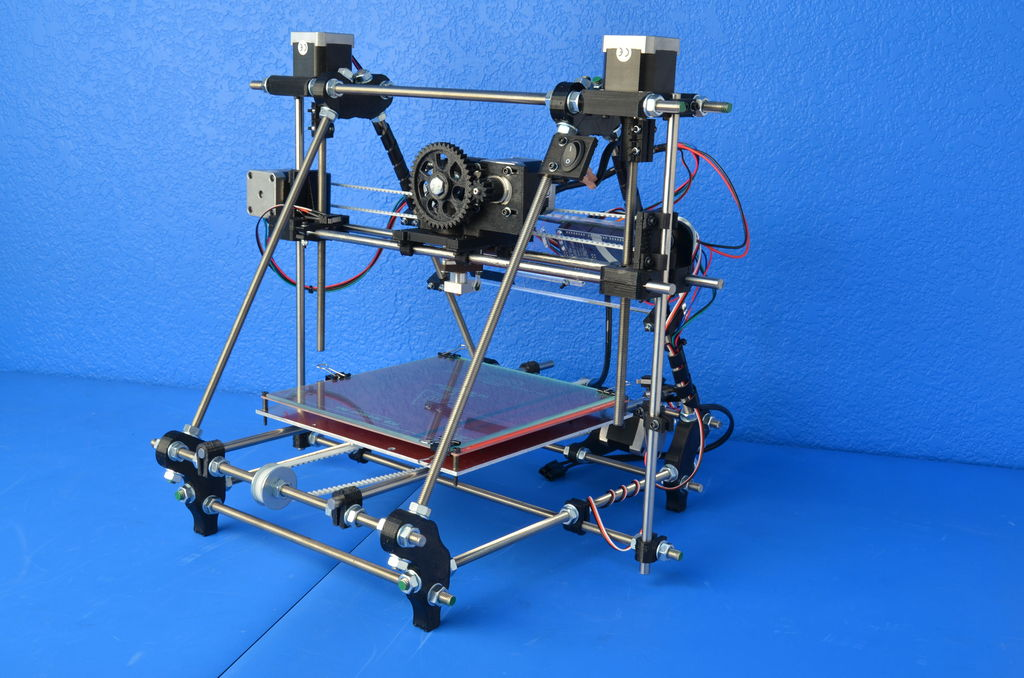
\includegraphics[keepaspectratio=true,height=0.40\textheight,width=1.00\textwidth,angle=0]{prusa/prusa-1-front-left.jpg}
 \caption{LulzBot Prusa 1.0 Front}
 \label{fig:prusa-1-front-left}
\end{figure}

\begin{figure}[h!]
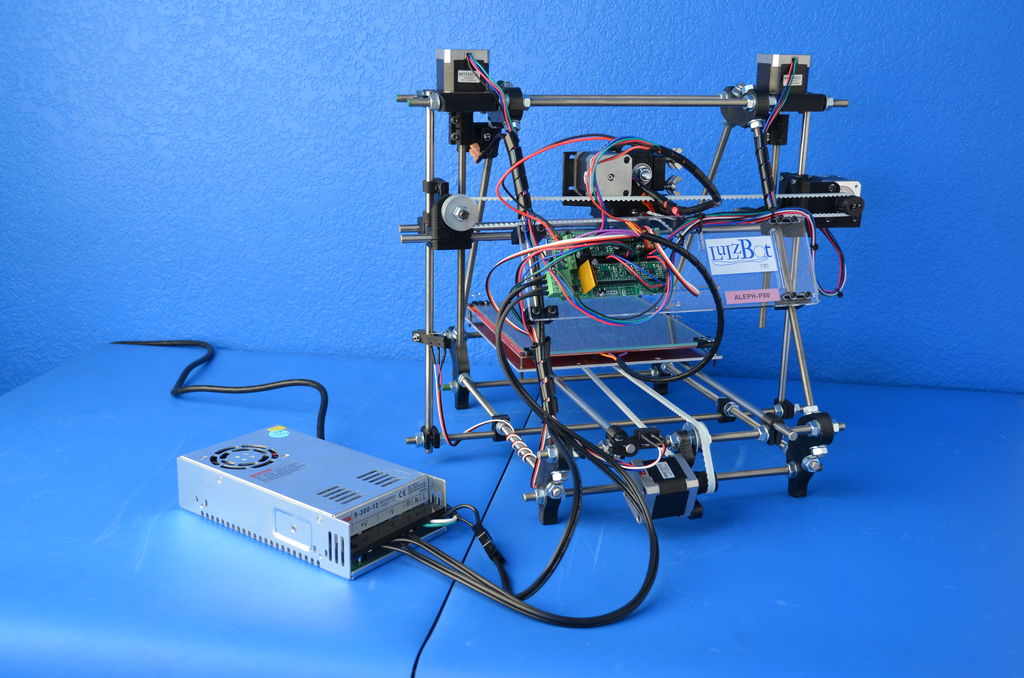
\includegraphics[keepaspectratio=true,height=0.40\textheight,width=1.00\textwidth,angle=0]{prusa/prusa-1-back.jpg}
 \caption{LulzBot Prusa 1.0 Back}
 \label{fig:prusa-1-back}
\end{figure}

\begin{figure}[h!]
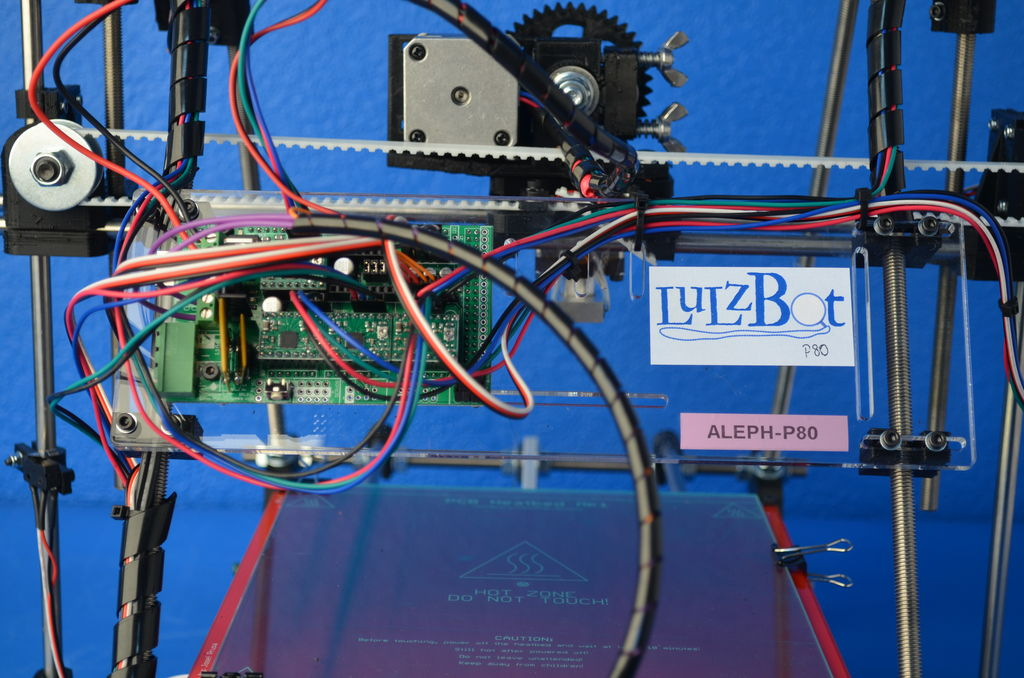
\includegraphics[keepaspectratio=true,height=0.40\textheight,width=1.00\textwidth,angle=0]{prusa/prusa-1-electronics.jpg}
 \caption{LulzBot Prusa 1.0 Electronics}
 \label{fig:prusa-1-electronics}
\end{figure}

\begin{figure}[h!]
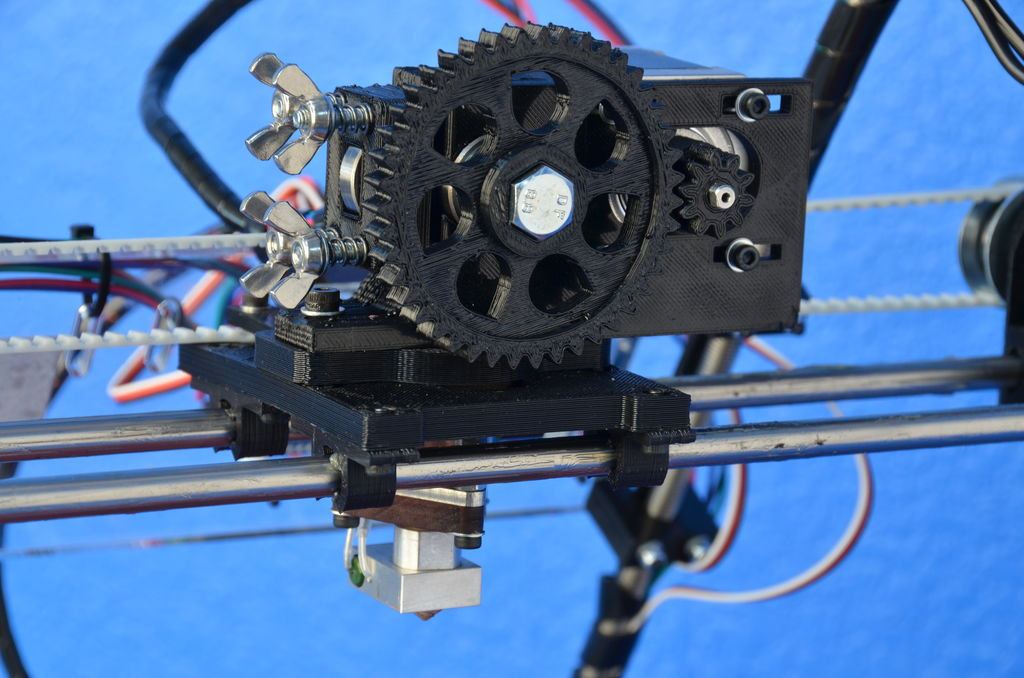
\includegraphics[keepaspectratio=true,height=0.40\textheight,width=1.00\textwidth,angle=0]{prusa/prusa-1-extruder.jpg}
 \caption{LulzBot Prusa 1.0 Extruder}
 \label{fig:prusa-1-extruder}
\end{figure}

\begin{figure}[h!]
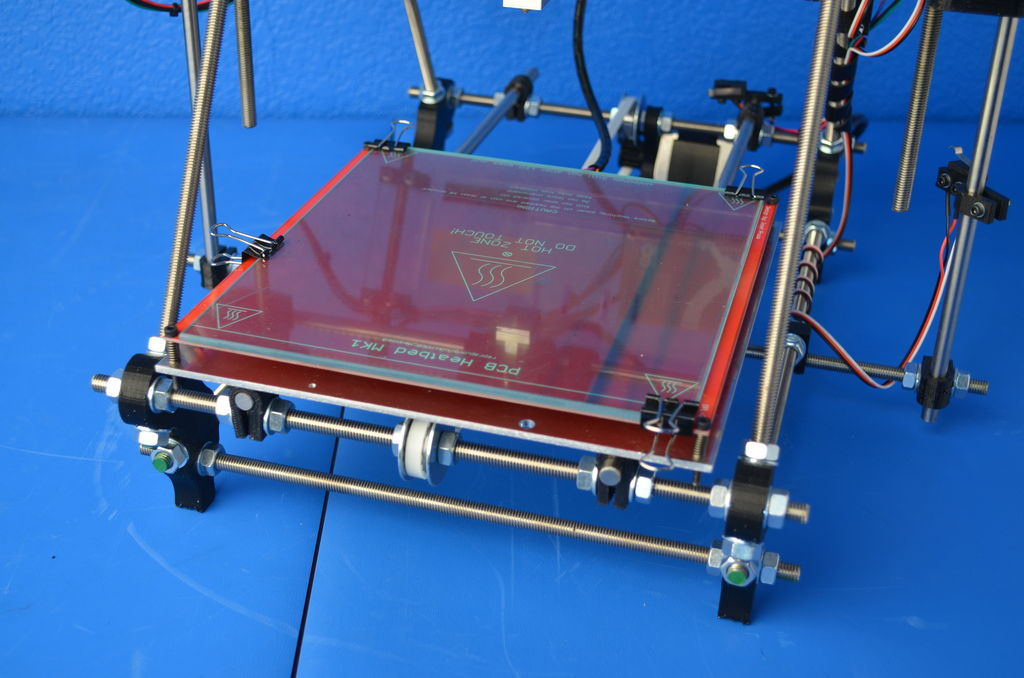
\includegraphics[keepaspectratio=true,height=0.40\textheight,width=1.00\textwidth,angle=0]{prusa/prusa-1-heatbed.jpg}
 \caption{LulzBot Prusa 1.0 Heatbed}
 \label{fig:prusa-1-heatbed}
\end{figure}

\begin{figure}[h!]
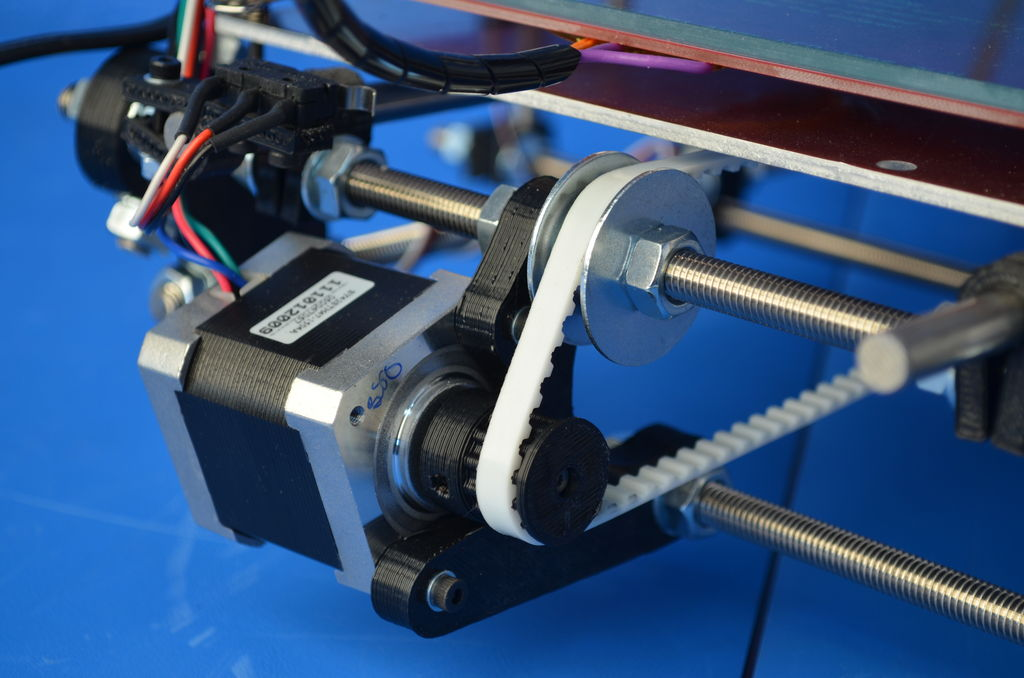
\includegraphics[keepaspectratio=true,height=0.40\textheight,width=1.00\textwidth,angle=0]{prusa/prusa-1-ybelt.jpg}
 \caption{LulzBot Prusa 1.0 Y Belt}
 \label{fig:prusa-1-ybelt}
\end{figure}

%\begin{figure}[h!]
%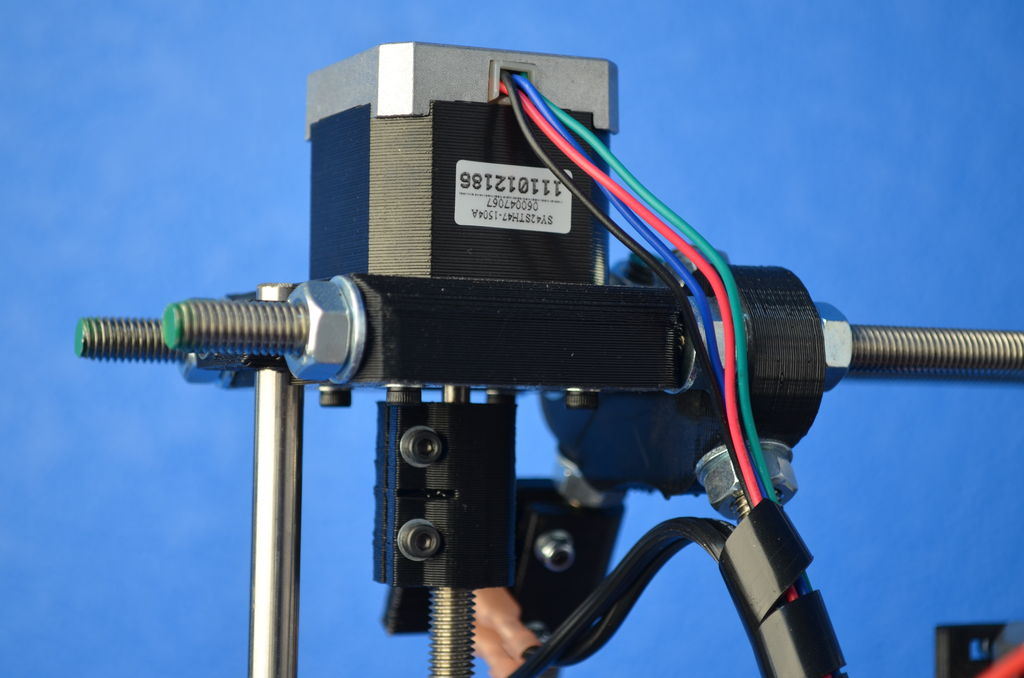
\includegraphics[keepaspectratio=true,height=0.40\textheight,width=1.00\textwidth,angle=0]{prusa/prusa-1-motor.jpg}
% \caption{LulzBot Prusa 1.0 Motor}
% \label{fig:prusa-1-motor}
%\end{figure}

%\begin{figure}[h!]
%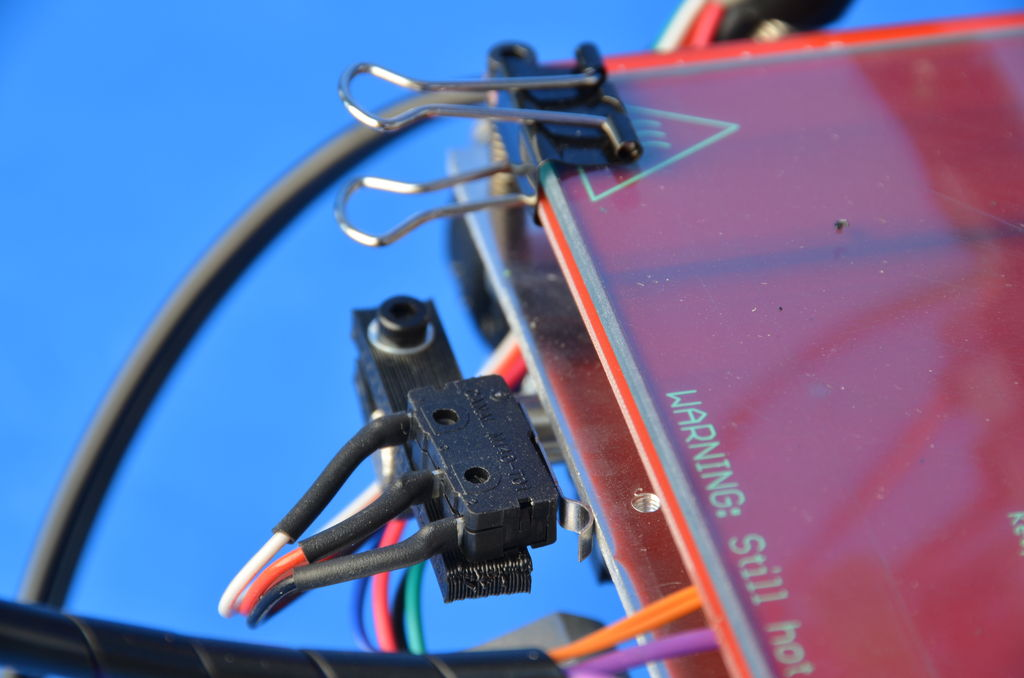
\includegraphics[keepaspectratio=true,height=0.40\textheight,width=1.00\textwidth,angle=0]{prusa/prusa-1-endstop.jpg}
% \caption{LulzBot Prusa 1.0 Endstop}
% \label{fig:prusa-1-endstop}
%\end{figure}

\begin{figure}[h!]
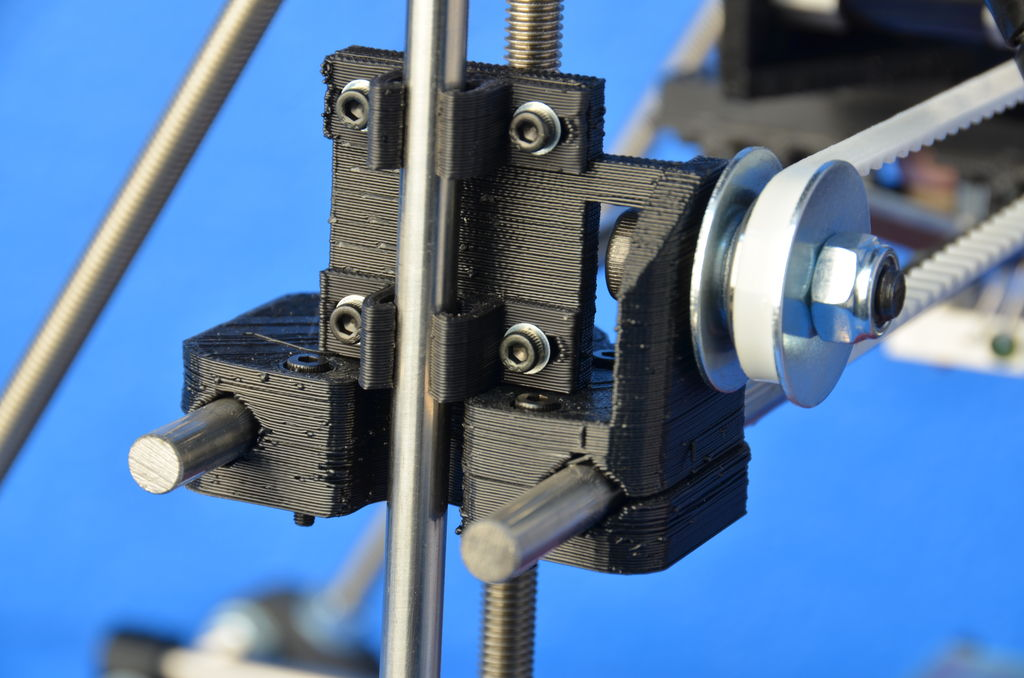
\includegraphics[keepaspectratio=true,height=0.40\textheight,width=1.00\textwidth,angle=0]{prusa/prusa-1-xend.jpg}
 \caption{LulzBot Prusa 1.0 X End}
 \label{fig:prusa-1-xend}
\end{figure}


%
% Prusa.tex
%
% History of LulzBot Printers
%
% Copyright (C) 2014, 2015 Aleph Objects, Inc.
%
% This document is licensed under the Creative Commons Attribution 4.0
% International Public License (CC BY-SA 4.0) by Aleph Objects, Inc.
%

\section{LulzBot Prusa 2.0}
LulzBot Prusa 2.0.

\begin{figure}[h!]
\thisfloatpagestyle{empty}
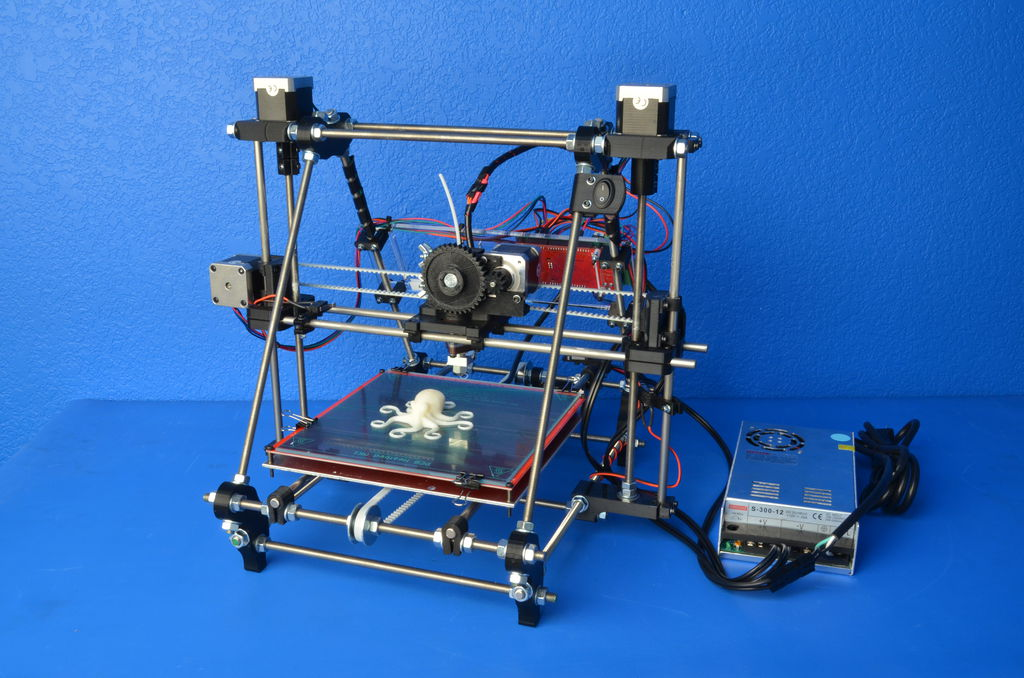
\includegraphics[keepaspectratio=true,height=0.40\textheight,width=1.00\textwidth,angle=0]{prusa/prusa-2-front-octo.jpg}
 \caption{LulzBot Prusa 2.0 Front with Octopus}
 \label{fig:prusa-2-front-octo}
\end{figure}

%\begin{figure}[h!]
%\thisfloatpagestyle{empty}
%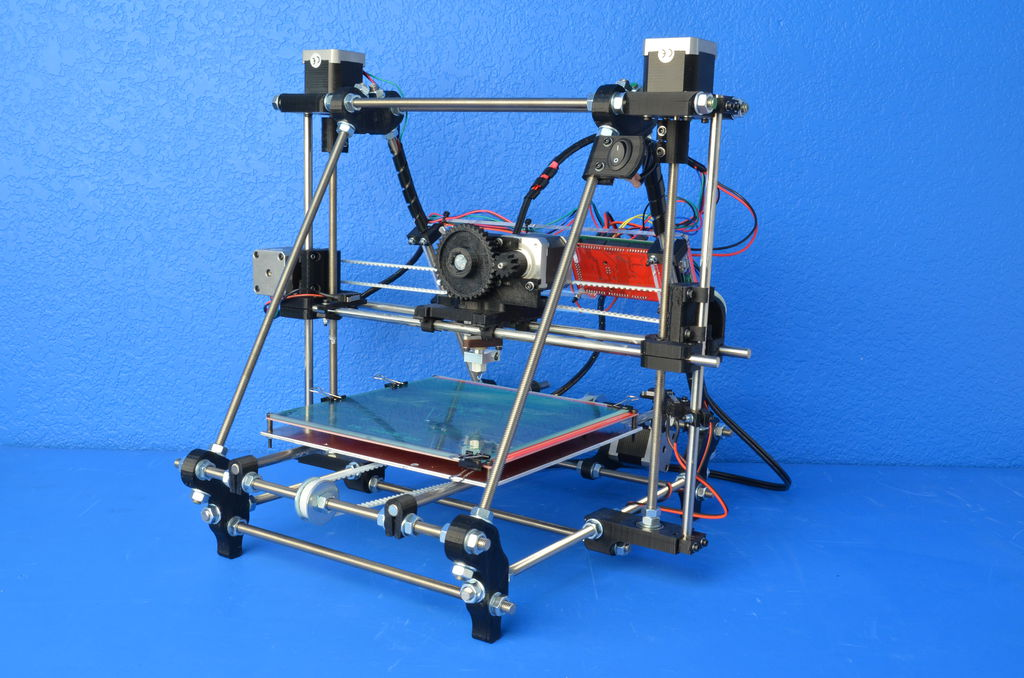
\includegraphics[keepaspectratio=true,height=0.40\textheight,width=1.00\textwidth,angle=0]{prusa/prusa-2-front.jpg}
% \caption{LulzBot Prusa 2.0 Front}
% \label{fig:prusa-2-front}
%\end{figure}

\begin{figure}[h!]
\thisfloatpagestyle{empty}
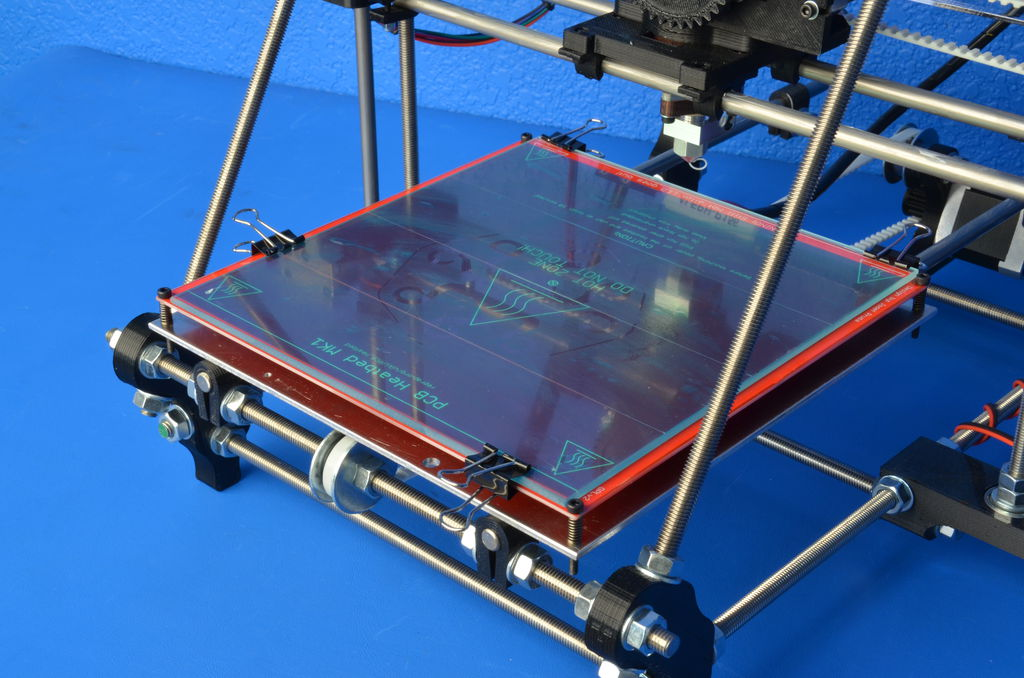
\includegraphics[keepaspectratio=true,height=0.40\textheight,width=1.00\textwidth,angle=0]{prusa/prusa-2-bed.jpg}
 \caption{LulzBot Prusa 2.0 Bed}
 \label{fig:prusa-2-bed}
\end{figure}

\begin{figure}[h!]
\thisfloatpagestyle{empty}
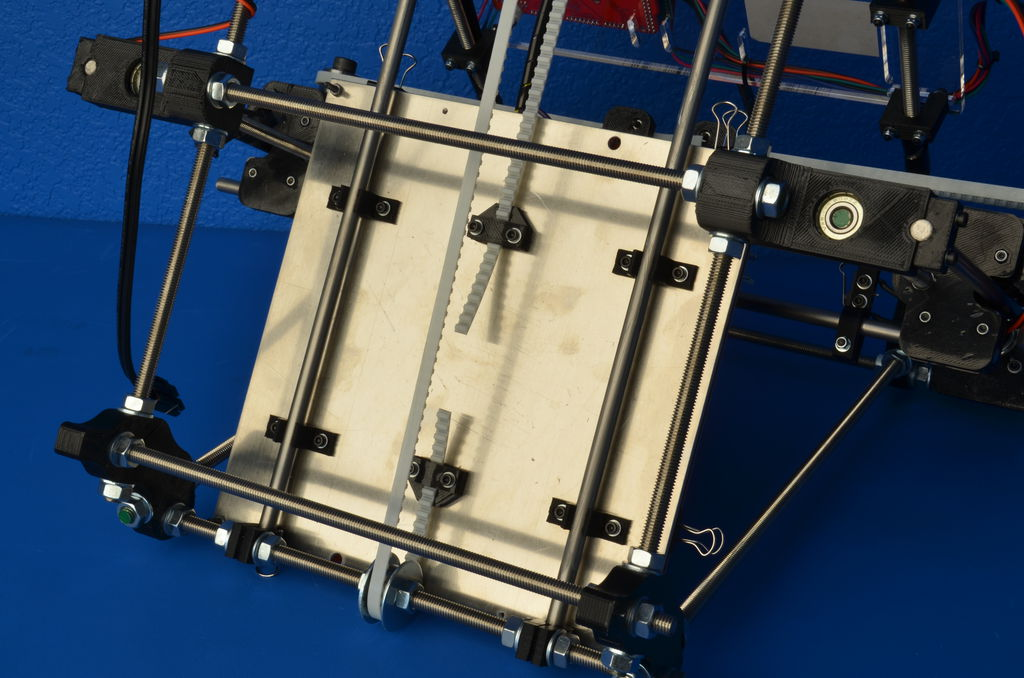
\includegraphics[keepaspectratio=true,height=0.40\textheight,width=1.00\textwidth,angle=0]{prusa/prusa-2-bottom.jpg}
 \caption{LulzBot Prusa 2.0 Bottom}
 \label{fig:prusa-2-bottom}
\end{figure}

\begin{figure}[h!]
\thisfloatpagestyle{empty}
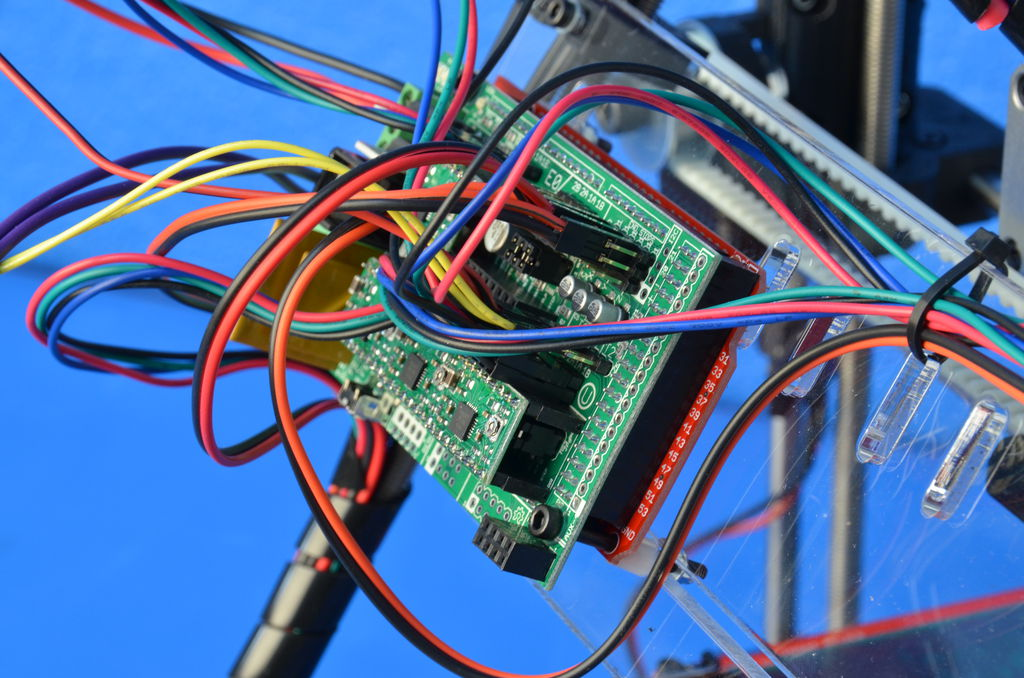
\includegraphics[keepaspectratio=true,height=0.40\textheight,width=1.00\textwidth,angle=0]{prusa/prusa-2-electronics.jpg}
 \caption{LulzBot Prusa 2.0 Electronics}
 \label{fig:prusa-2-electronics}
\end{figure}

%\begin{figure}[h!]
%\thisfloatpagestyle{empty}
%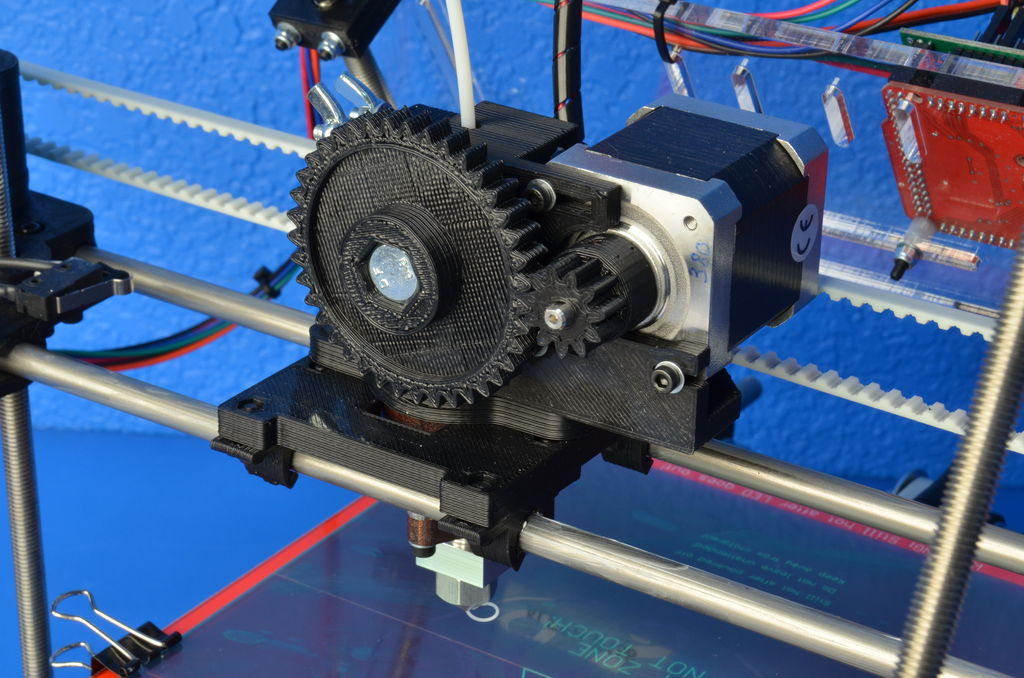
\includegraphics[keepaspectratio=true,height=0.40\textheight,width=1.00\textwidth,angle=0]{prusa/prusa-2-extruder2.jpg}
% \caption{LulzBot Prusa 2.0 Extruder}
% \label{fig:prusa-2-extruder2}
%\end{figure}

\begin{figure}[h!]
\thisfloatpagestyle{empty}
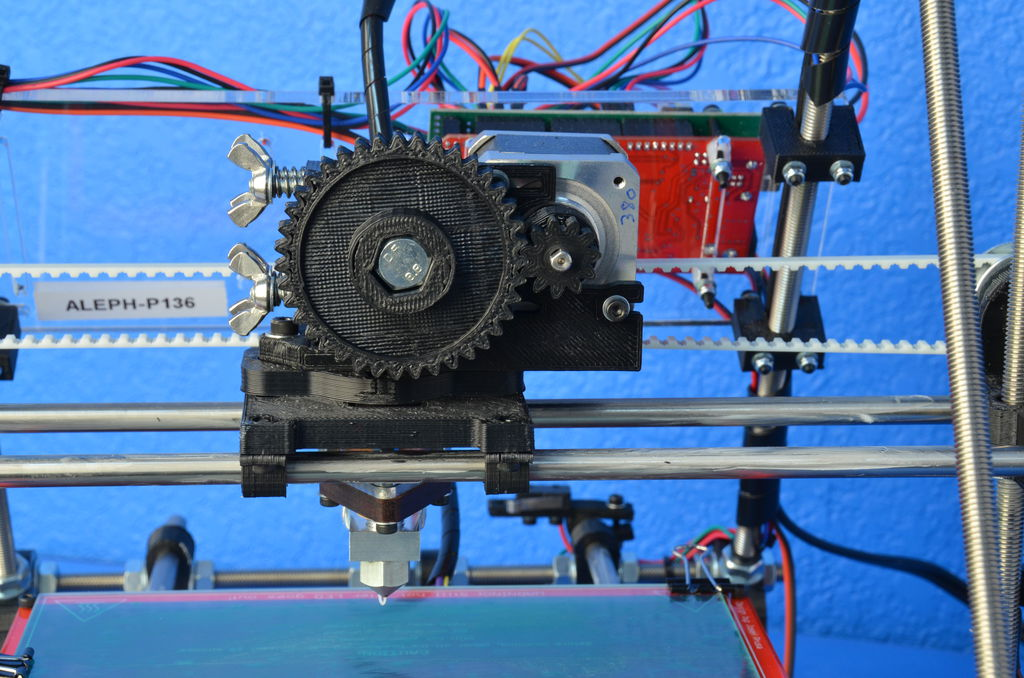
\includegraphics[keepaspectratio=true,height=0.40\textheight,width=1.00\textwidth,angle=0]{prusa/prusa-2-extruder.jpg}
 \caption{LulzBot Prusa 2.0 Extruder}
 \label{fig:prusa-2-extruder}
\end{figure}

\begin{figure}[h!]
\thisfloatpagestyle{empty}
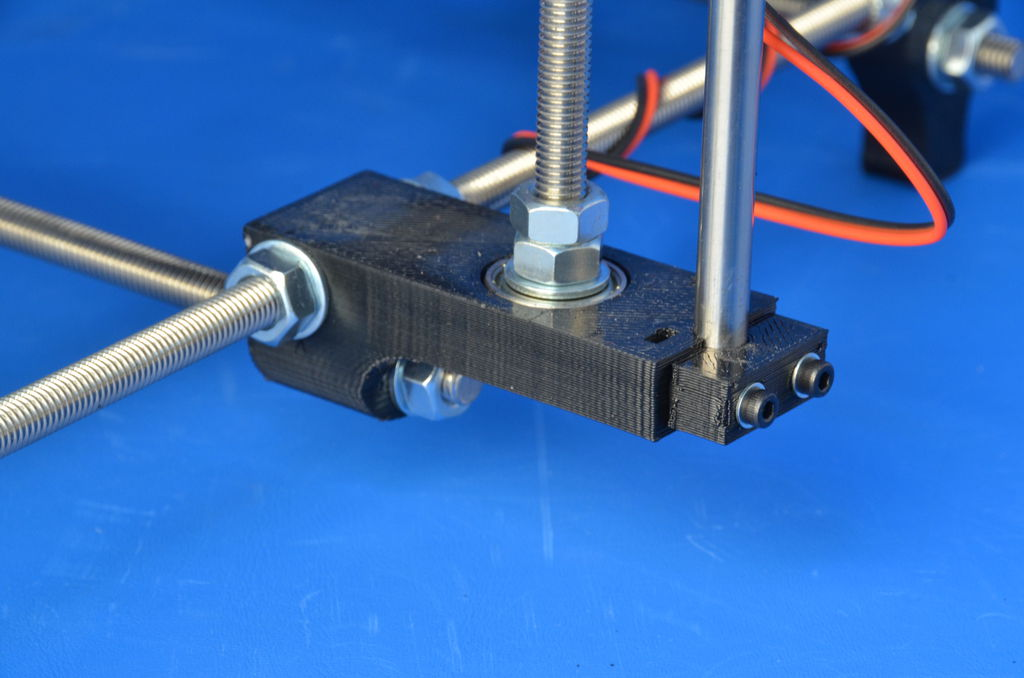
\includegraphics[keepaspectratio=true,height=0.40\textheight,width=1.00\textwidth,angle=0]{prusa/prusa-2-mount.jpg}
 \caption{LulzBot Prusa 2.0 Mount}
 \label{fig:prusa-2-mount}
\end{figure}

\begin{figure}[h!]
\thisfloatpagestyle{empty}
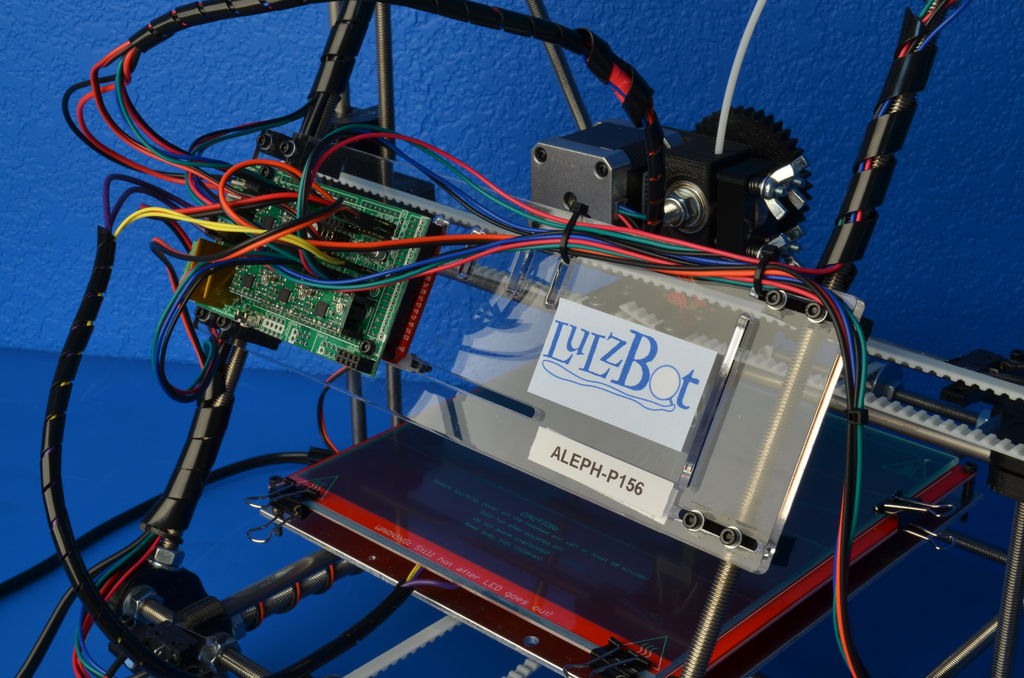
\includegraphics[keepaspectratio=true,height=0.40\textheight,width=1.00\textwidth,angle=0]{prusa/prusa-2-panel.jpg}
 \caption{LulzBot Prusa 2.0 Panel}
 \label{fig:prusa-2-panel}
\end{figure}

%\begin{figure}[h!]
%\thisfloatpagestyle{empty}
%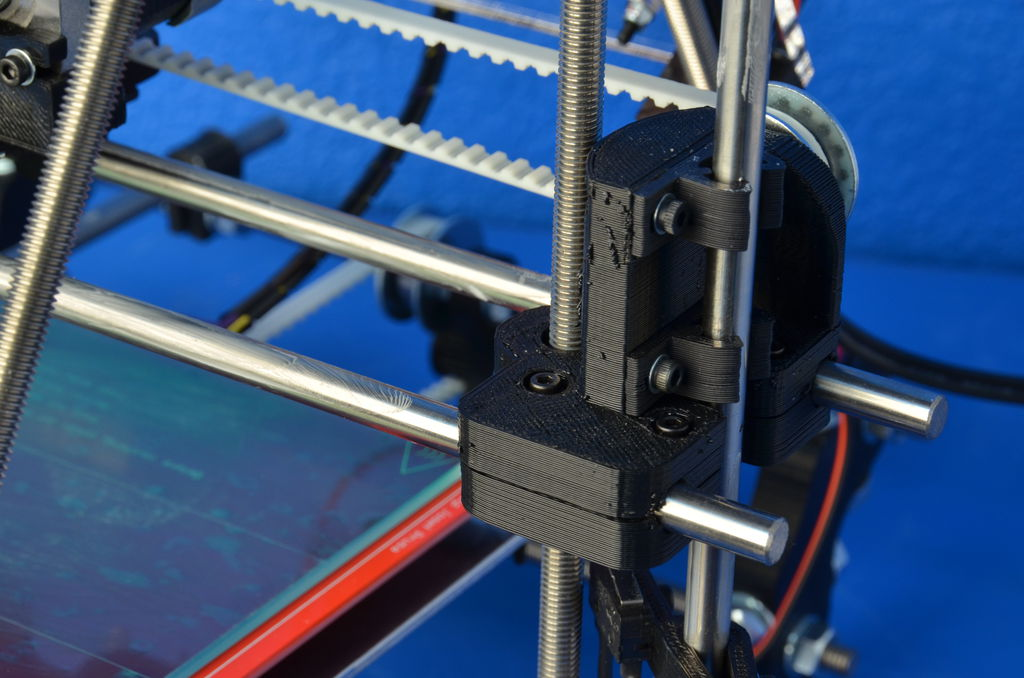
\includegraphics[keepaspectratio=true,height=0.40\textheight,width=1.00\textwidth,angle=0]{prusa/prusa-2-xidler.jpg}
% \caption{LulzBot Prusa 2.0 X Idler}
% \label{fig:prusa-2-xidler}
%\end{figure}

%\begin{figure}[h!]
%\thisfloatpagestyle{empty}
%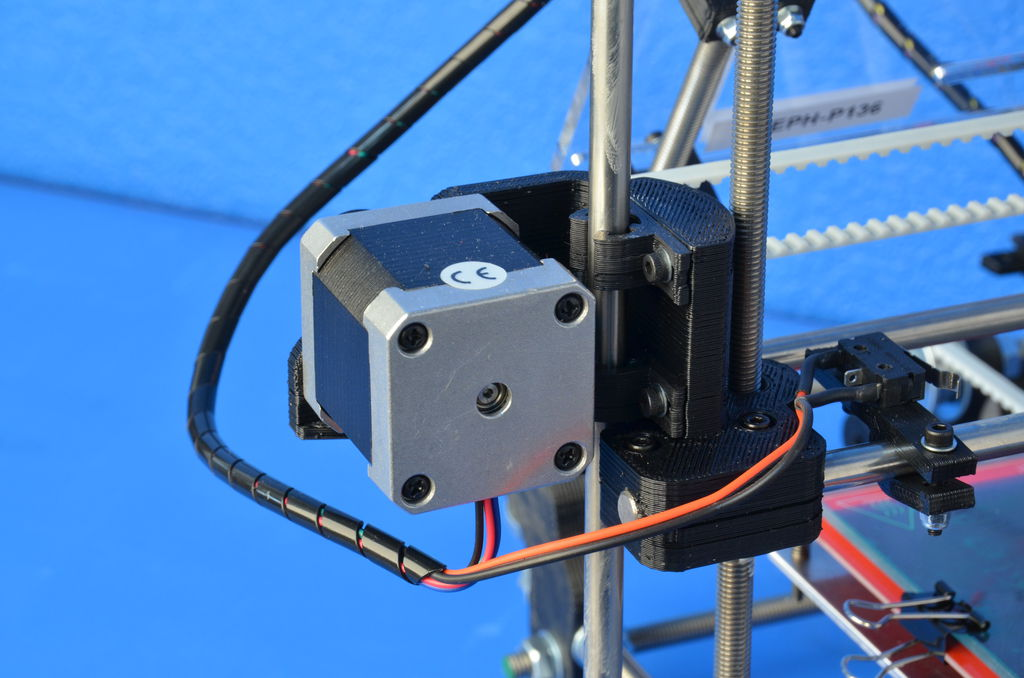
\includegraphics[keepaspectratio=true,height=0.40\textheight,width=1.00\textwidth,angle=0]{prusa/prusa-2-xmotor.jpg}
% \caption{LulzBot Prusa 2.0 X Motor}
% \label{fig:prusa-2-xmotor}
%\end{figure}



